\chapter{MR-WPT回路の原理}
\section{MR-WPT回路の特性}
磁界共鳴方式無線電力伝送(Magnetic Resonance Wireless Power Transfer : MR-WPT)回路は,図\ref{mr-wpt}のように,相互インダクタンス$M$で結合した送電コイル$L_1$と受電コイル$L_2$に,それぞれ共振用のキャパシタ$C_1$ならびに$C_2$を付加することにより,大電力かつ高効率の電力伝送を実現するものである\cite{Imura2017}.ここで,$L_1, \, C_1$の積と$L_2, \, C_2$の積の値とは等しくなるよう設計する.共振用キャパシタの接続方法(直列あるいは並列)により数種類の回路構成があるが,本稿では,図\ref{mr-wpt}のように2つの共振用キャパシタを送受電コイルに対していずれも直列に挿入する回路を扱う.\par 

\begin{figure}[b]
\begin{center}

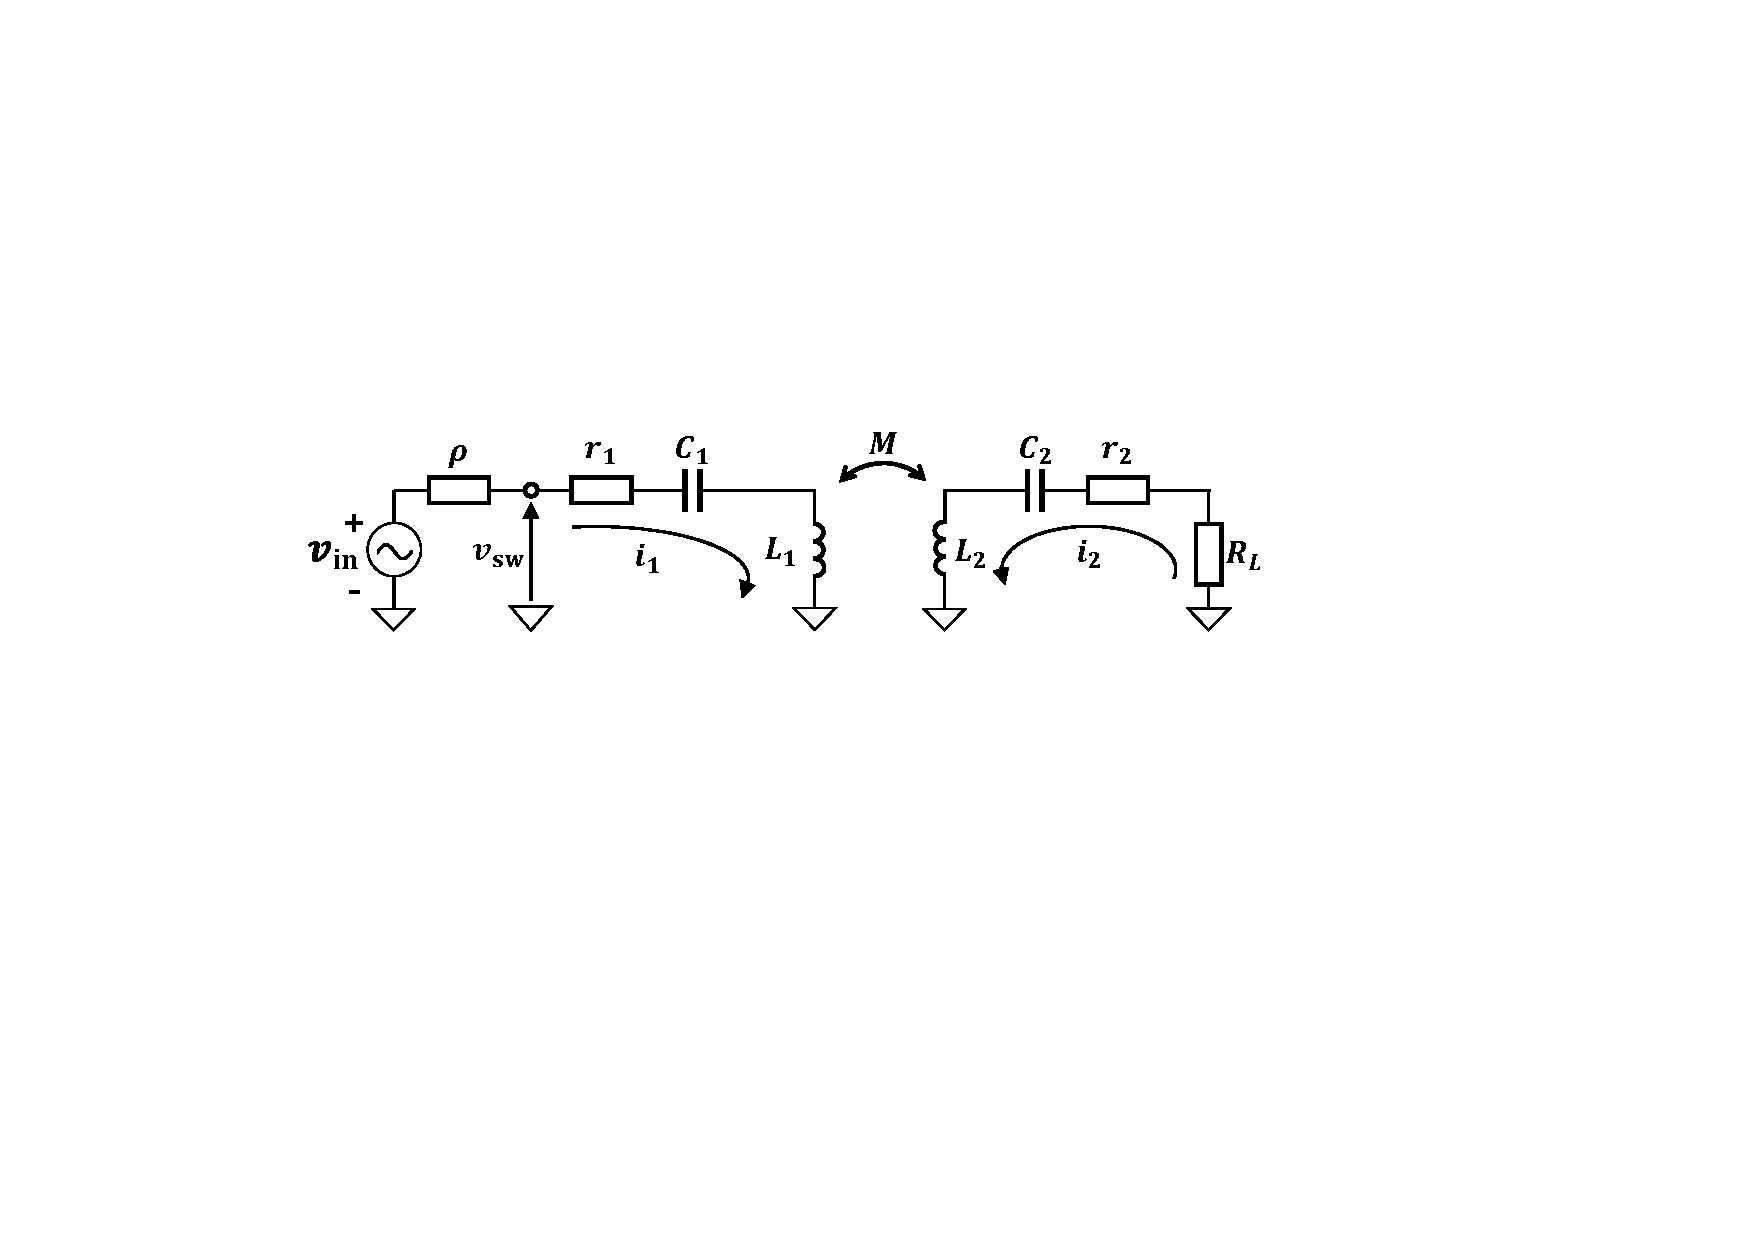
\includegraphics[width=130mm]{figures/mr-wpt.pdf}
\caption{MR-WPT回路}
\label{mr-wpt}
\end{center}

\end{figure}

図\ref{mr-wpt}に示す回路の動作を解析する.同図において,$v_{in}$は入力電源の開放電圧,$i_1,i_2$はループ電流,$L_1,L_2$は送受電コイルの自己インダクタンス,$M$は$L_1,L_2$の相互インダクタンス,$C_1,C_2$は送・受電それぞれの回路での共振に必要なキャパシタの値,$\rho$は入力電源の出力抵抗,$r_1$は$L_1,C_1$のESRの和,$r_2$は$L_2,C_2$のESRの和であり,$R_L$は負荷抵抗である.ここで,回路解析のために,$L_1$と$L_2$からなる変成器をT型等価回路を用いて変形すると図\ref{equivalent}のようになり,ループ電流$i_1$ならびに$i_2$についてKVLを適用すれば

\begin{equation}
\begin{pmatrix}
v_{in}\\
0\\
\end{pmatrix} 
=
\begin{pmatrix}
\rho+r_1+j\left(\omega L_1 -\frac{1}{\omega C_1}\right) & -j\omega M \\
-j\omega M & r_2+R_L+j\left(\omega L_2 -\frac{1}{\omega C_2}\right)
\end{pmatrix}
\begin{pmatrix}
i_1 \\
i_2\\\end{pmatrix}
\end{equation}

となる.上式を$i_1$ならびに$i_2$について解くことにより,回路電流の解析解

\begin{equation}
\begin{pmatrix}
i_1 \\
i_2 \\
\end{pmatrix}
=
\frac{v_{in}}{D(j\omega)} \cdot
\begin{pmatrix}
r_2+R_L+j(\omega L_2 -\frac{1}{\omega C_2}) \\
-j\omega M \\
\end{pmatrix}
\end{equation}
が得られる.ここで,
\begin{equation}
D(j\omega)=\left\{\rho+r_1+j\left(\omega L_1 -\frac{1}{\omega C_1}\right)\right\} \cdot \left\{{r_2+R_L+j\left(\omega L_2 -\frac{1}{\omega C_2}\right)}\right\}+\omega^2 M^2
\end{equation}
である.式(2.2)より,電圧源$v_{in}$から右側を見た回路全体のインピーダンス$Z_{in}=v_{in}/i_1$は,
\begin{equation}
Z_{in}=\frac{D(j\omega)}{r_2+R_L+j\left(\omega L_2 -\frac{1}{\omega C_2}\right)}
\end{equation}
であり,回路全体を入力電源から見たインピーダンス$v_{sw}/i_1$は$Z_{in}-\rho$と表わせる.\par

\begin{figure}[b]
\begin{center}

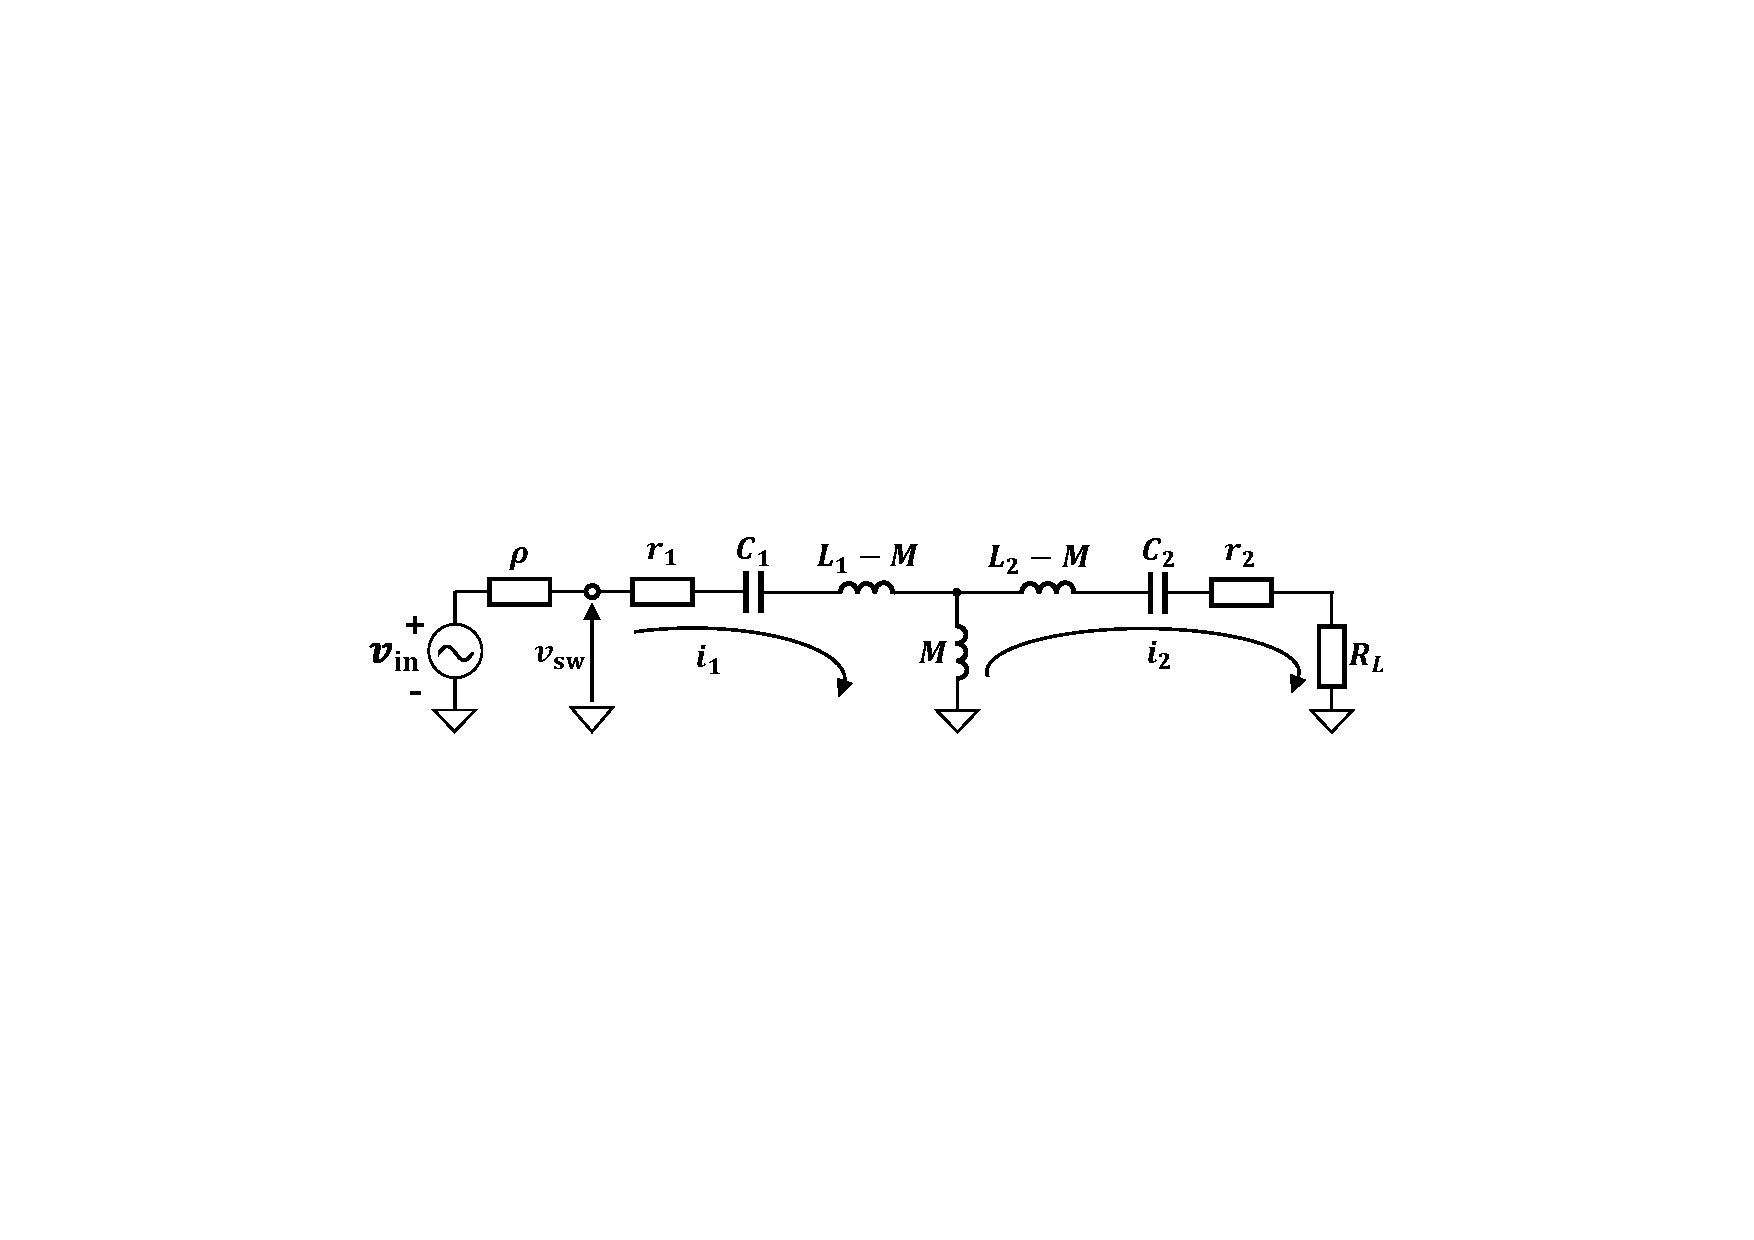
\includegraphics[width=130mm]{figures/equivalent.pdf}
\caption{MR-WPTのT型等価回路}
\label{equivalent}
\end{center}

\end{figure}

\begin{table}[t]
\centering
\caption{MR-WPTの設計例}
\begin{tabular}{c|r}
\hline
Circuit Parameter & \multicolumn{1}{c}{Value} \\ \hline \hline
$L_1,L_2$             & 5 $ \mathrm{\mu H}$  \\ \hline
$C_1,C_2$             & 0.01 $ \mathrm{\mu F}$ \\ \hline
$\rho+r_1$           & 0.1 $ \mathrm{\Omega}$ \\ \hline
$r_2$           & 0.1 $ \mathrm{\Omega}$ \\ \hline
$R_L$                 & 5 $ \mathrm{\Omega}$ \\ \hline
$v_{in}$               & $5\ \rm V_{\rm RMS}$ \\ \hline
\end{tabular}
\end{table}

\begin{figure}[h]

	\begin{center}
    \subfloat[$M= 2.5\, \mathrm{\mu H}$]{
    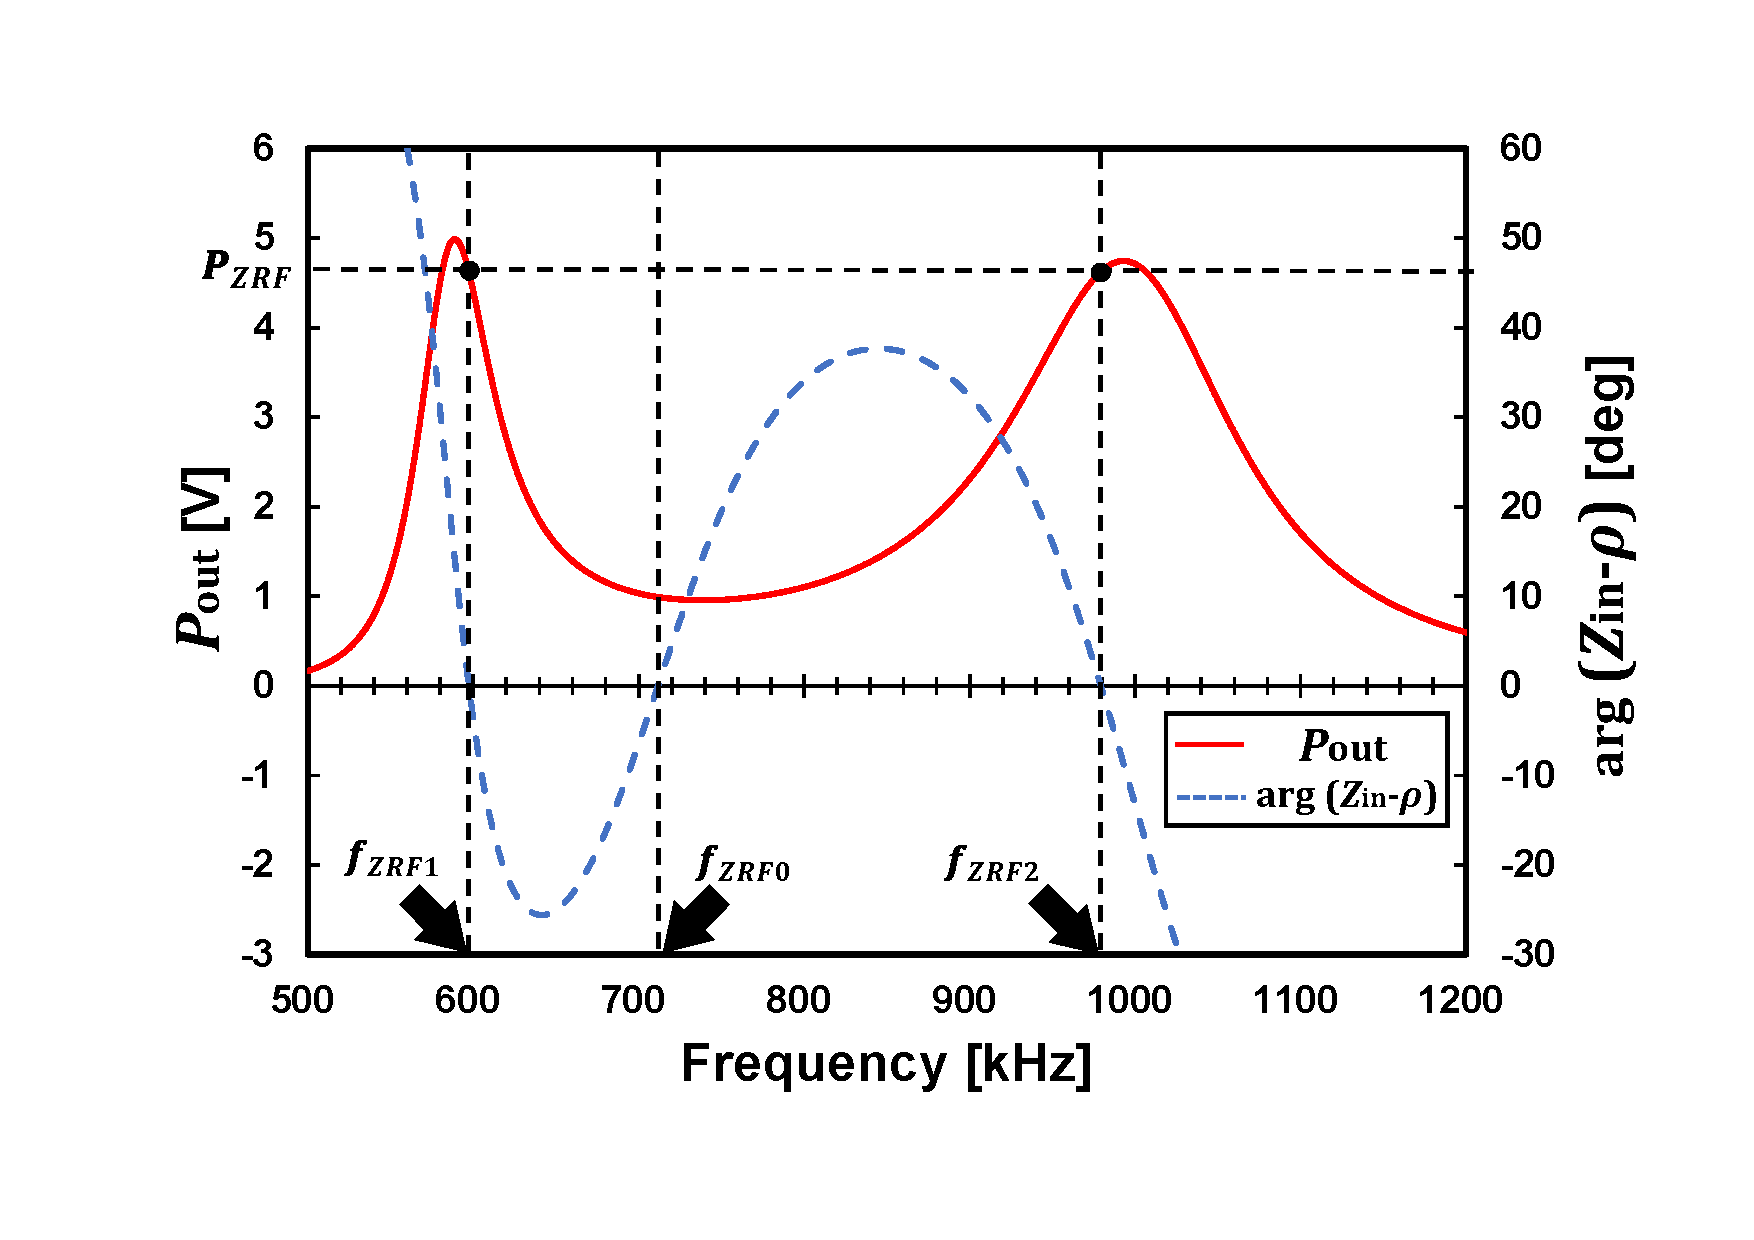
\includegraphics[width=75mm]{figures/freqchar05.pdf}
    }
    \subfloat[$M= 1.5\, \mathrm{\mu H}$]{
    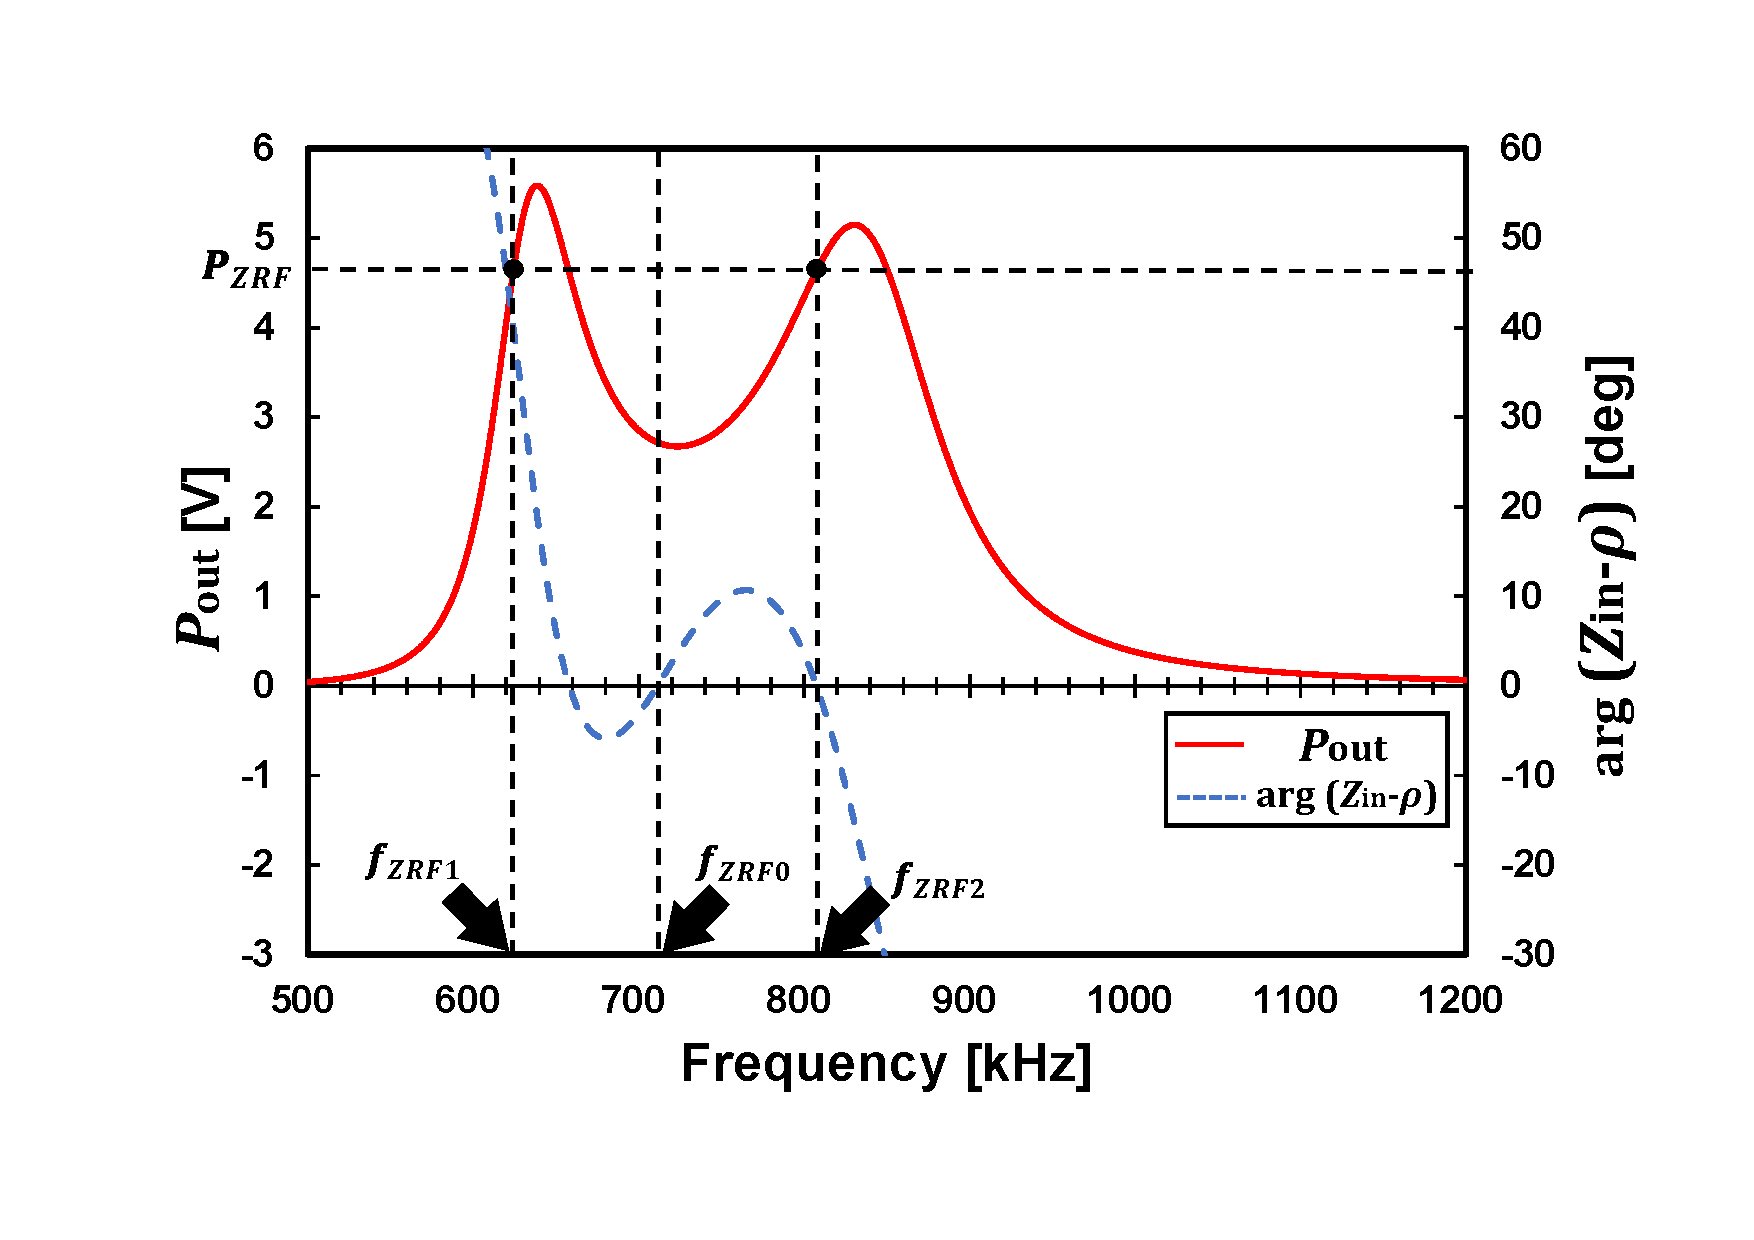
\includegraphics[width=75mm]{figures/freqchar03.pdf}
    }
    \end{center}
  \caption{MR-WPTの周波数特性}\label{freqchar}
\end{figure}

ここで,設計例を表2.1に示す.同表の数値と式(2.2)-(2.4)を用いて,負荷抵抗$R_L$で消費される電力$P_{out}=|i_2|^2 \cdot R_L$と,インピーダンス$Z_{in}-\rho$の位相特性$\arg(Z_{in}-\rho)$とを数値計算した結果を図\ref{freqchar}(a),(b)に示す.ただし,伝送コイル間の相互インダクタンス$M$は$2.5 \, \mathrm{\mu H}$ならびに$1.5 \, \mathrm{\mu H}$とした.図\ref{freqchar}には,出力電力が極大となる周波数,すなわ極大電力周波数が2つ存在する.これは,Frequency Splitting PhenomenaあるいはBifurcation Phenomenaとして知られている現象である\cite{Wang2004,Hoeher2019,Niu2013}.また,インピーダンス$Z_{in}-\rho$の位相特性が零になる周波数(Zero Reactance Frequency : ZRF)が3つ存在している.3つのZRFのうち,周波数軸上の左端と右端にある$f_{ZRF1}$, $f_{ZRF2}$は,2つの極大電力周波数の近傍にある.さらに,図\ref{freqchar}(a),(b)の対比から,ZRFならびに極大電力周波数の値はコイル間の相互インダクタンス$M$に依存することが分かる.\par 
以上より,MR-WPT回路で大電力を伝送したい場合,回路をいずれかの極大電力周波数で駆動しなければならないことが分かる.さらに個々の回路素子の値が不変であるという条件下において,コイル間の相互インダクタンスが変動するような用途を想定した場合,何らかの方法で極大電力周波数を追従する回路が必要になる.文献\cite{Fujita2019a}においては,ZRFが極大電力周波数の近傍にあることに着目し,ZRFを追従することで等価的に極大電力周波数を追従する手法について提案した.同手法については,3章で詳しく述べる.

\section{ZRFの解析}
\subsection{ZRFの解析式}
前項においては,ZRFが極大電力周波数の自動追従という観点から重要であることを示唆した.本項では,前項における回路解析の結果を用いてZRFの解析式を導出するとともに,ZRFで回路を駆動する際の特性について検討する.\par 
ZRFは,MR-WPT回路を入力電源から見たインピーダンス$Z_{in}-\rho$の位相特性が零になる周波数,すなわち$Z_{in}-\rho$のリアクタンス成分が零になる周波数であるから,それを求めるには,$\rho$が実数であることに留意すれば
\begin{equation}
\Im[Z_{in}]=0
\end{equation}
なる方程式を角周波数$\omega$について解けばよい.上式をそのまま求解するのは極めて煩雑であるから,送受電回路が対称である,すなわち
\begin{gather}
r_1+\rho = r_2=r, \, C_1=C_2=C, \, L_1=L_2=L
\end{gather}
と仮定する.このとき,式(2.3),(2.4)より
\begin{align}
Z_{in} &=\frac{D(j\omega)}{r_2+R_L+j\left(\omega L_2 -\frac{1}{\omega C_2}\right)} \\
&=\cfrac{\left\{r+j\left(\omega L -\frac{1}{\omega C}\right)\right\} \cdot \left\{{r+R_L+j\left(\omega L -\frac{1}{\omega C}\right)}\right\}+\omega^2 M^2}{r+R_L+j\left(\omega L -\frac{1}{\omega C}\right)} \\
&=r+j\left(\omega L -\frac{1}{\omega C}\right)+\frac{\omega^2 M^2}{r+R_L+j\left(\omega L -\frac{1}{\omega C}\right)} \\
&=r+\frac{\omega^2 M^2(r+R_L)}{(r+R_L)^2+\left(\omega L -\frac{1}{\omega C}\right)^2}+j\left(\omega L -\frac{1}{\omega C}-\frac{\omega^2 M^2 \left(\omega L -\frac{1}{\omega C}\right)}{(r+R_L)^2+\left(\omega L -\frac{1}{\omega C}\right)^2}\right)
\end{align}
である.したがって,式(2.5)は
\begin{equation}
\Im[Z_{in}]=0 \leftrightarrow \omega L -\frac{1}{\omega C}=\frac{\omega^2 M^2 \left(\omega L -\frac{1}{\omega C}\right)}{(r+R_L)^2+\left(\omega L -\frac{1}{\omega C}\right)^2}
\end{equation}
となる.\par 
式(2.11)は,
\begin{equation}
\omega L -\frac{1}{\omega C}=0 \leftrightarrow \omega=\frac{1}{\sqrt{LC}} \leftrightarrow f=\frac{1}{2\pi \sqrt{LC}}
\end{equation}
のとき明らかに成立する.ただし,$\omega=2 \pi f$の関係を用いた.よって,式(2.12)は式(2.11)のひとつの解であり,図\ref{freqchar}における$f_{ZRF0}$に対応する.$\omega \neq 1/\sqrt{LC}$のとき,式(2.11)は
\begin{align}
1&=\frac{\omega^2 M^2}{(r+R_L)^2+\left(\omega L -\frac{1}{\omega C}\right)^2} \\
\omega^2 M^2 &=(r+R_L)^2+\omega^2 L^2-2\frac{L}{C}+\frac{1}{\omega^2 C^2} \\
0&=\omega^4(C^2L^2-C^2M^2)+\omega^2 \left\{C^2(r+R_L)^2-2LC\right\}+1
\end{align}
となる.これは$\omega$に関する複2次式であるから,2次方程式の解の公式を用いて解くことができる.得られる4つの解のうち,正のものを$\omega_{ZRF1}, \, \omega_{ZRF2} \, (\omega_{ZRF1}<\omega_{ZRF2})$として,さらに$M=k\sqrt{L_1L_2}=k\sqrt{L^2}=kL$の関係を用いれば
\begin{equation}
\omega_{ZRF1}
=\sqrt{\frac{2L-C(r+R_L)^2 - \sqrt{C^2(r+R_L)^4-4LC(r+R_L)^2+4M^2}}{2CL^2(1-k^2)}} 
\end{equation}
\begin{equation}
\omega_{ZRF2}
=\sqrt{\frac{2L-C(r+R_L)^2 + \sqrt{C^2(r+R_L)^4-4LC(r+R_L)^2+4M^2}}{2CL^2(1-k^2)}} 
\end{equation}
となる.これらは共役関係であり,両角周波数におけるMR-WPT回路の出力電力$P_{out}=|i_2|^2 \cdot R_L$は等しい.
式(2.16),(2.17)に表1の数値例ならびに$k=0.5\, (M=2.5 \, \mathrm{\mu H})$を代入し,$2\pi$で除算することにより2つのZRF$f_{ZRF1},f_{ZRF2}$を求めると,
\begin{align}
f_{ZRF1} \simeq 597.4 \, \mathrm{kHz} \\
f_{ZRF2} \simeq 979.3 \, \mathrm{kHz}
\end{align}
となる.これは,図\ref{freqchar}(a)に示した$f_{ZRF1},f_{ZRF2}$と対応する.\par 
図\ref{zrfgraph}は,式(2.12),(2.16)ならびに式(2.17)から,コイル間結合係数$k$と各ZRFの関係を数値計算した結果である.同図より,$f_{ZRF1}, \, f_{ZRF2}$は,$k>k_{th}$のとき存在し,$k$に依存して変動する.結合係数$k$のしきい値$k_{th}$は次項で導出する.

\subsection{ZRFが複数存在する条件}
図\ref{zrfgraph}に示したとおり,$f_{ZRF1}, f_{ZRF2}$は結合係数$k$があるしきい値$k_{th}$より大きいときに存在する.$k_{th}$は,式(2.16),(2.17)が実数値をとる範囲を導出することにより求められる.ここでは,例として式(2.17)について考える.同式が実数となるための必要十分条件は,結合係数$k$が定義される範囲$0<k<1$において分母が常に正であることを考慮すると
\begin{equation}
2L-C(r+R_L)^2 + \sqrt{C^2(r+R_L)^4-4LC(r+R_L)^2+4k^2L^2} \geq 0
\end{equation}
である.これを満たすためには,

\begin{subnumcases}
{}
C^2(r+R_L)^4-4LC(r+R_L)^2+4k^2L^2 \geq 0 &\\
C(r+R_L)^2-2L \geq 0 &\\
C^2(r+R_L)^4-4LC(r+R_L)^2+4k^2L^2 \geq \left\{C(r+R_L)^2-2L\right\}^2 &
\end{subnumcases}
または
\begin{subnumcases}
{}
C^2(r+R_L)^4-4LC(r+R_L)^2+4k^2L^2 \geq 0 \\
C(r+R_L)^2-2L \leq 0
\end{subnumcases}
であればよい.ここで,式(2.21c)を整理すると
\begin{align}
C^2(r+R_L)^4-4LC(r+R_L)^2+4k^2L^2 &\geq \left\{C(r+R_L)^2-2L\right\}^2 \\
4k^2L^2 &\geq 4L^2 \\
k^2 \geq 1 \leftrightarrow &k\geq 1, \,  k\leq -1
\end{align}
となる.結合係数$k$が定義される範囲は$0<k<1$であり,したがって式(2.21)で示される条件は不適である.一方,式(2.22a)を$k$について解くと
\begin{align}
4k^2L^2 &\geq 4LC(r+R_L)^2-C^2(r+R_L)^4 \\
k^2 &\geq\frac{C}{L}(r+R_L)^2 \left(1-\frac{C}{4L}(r+R_L)^2\right) \\
k &\geq(r+R_L)\sqrt{\frac{C}{L}\left(1-\frac{C}{4L}(r+R_L)^2 \right)}
\end{align}
となる.また,式(2.22b)を負荷抵抗$R_L$について解けば
\begin{align}
C(r+R_L)^2 &\leq 2L \\
R_L &\leq \sqrt{\frac{2L}{C}}-r
\end{align}
となる.ここでは式(2.17)について述べたが,式(2.16)についても同様の結果が得られる.以上より,$f_{ZRF1}$,$f_{ZRF2}$が存在する,すなわちZRFが複数存在する条件は
\begin{equation}
k \geq k_{th}=(r+R_L)\sqrt{\frac{C}{L}\left(1-\frac{C}{4L}(r+R_L)^2 \right)} \, \,  \mbox{かつ} R_L \leq \sqrt{\frac{2L}{C}}-r
\end{equation}
と書ける.この条件を図示したものを図\ref{boundary}に示す.色付きの部分が,不等式(2.31)を満たす領域である.同図より,負荷抵抗$R_L$が大きいほど,複数のZRFが得られる結合係数$k$の範囲は狭くなることが分かる.
\begin{figure}[h]
\begin{center}

        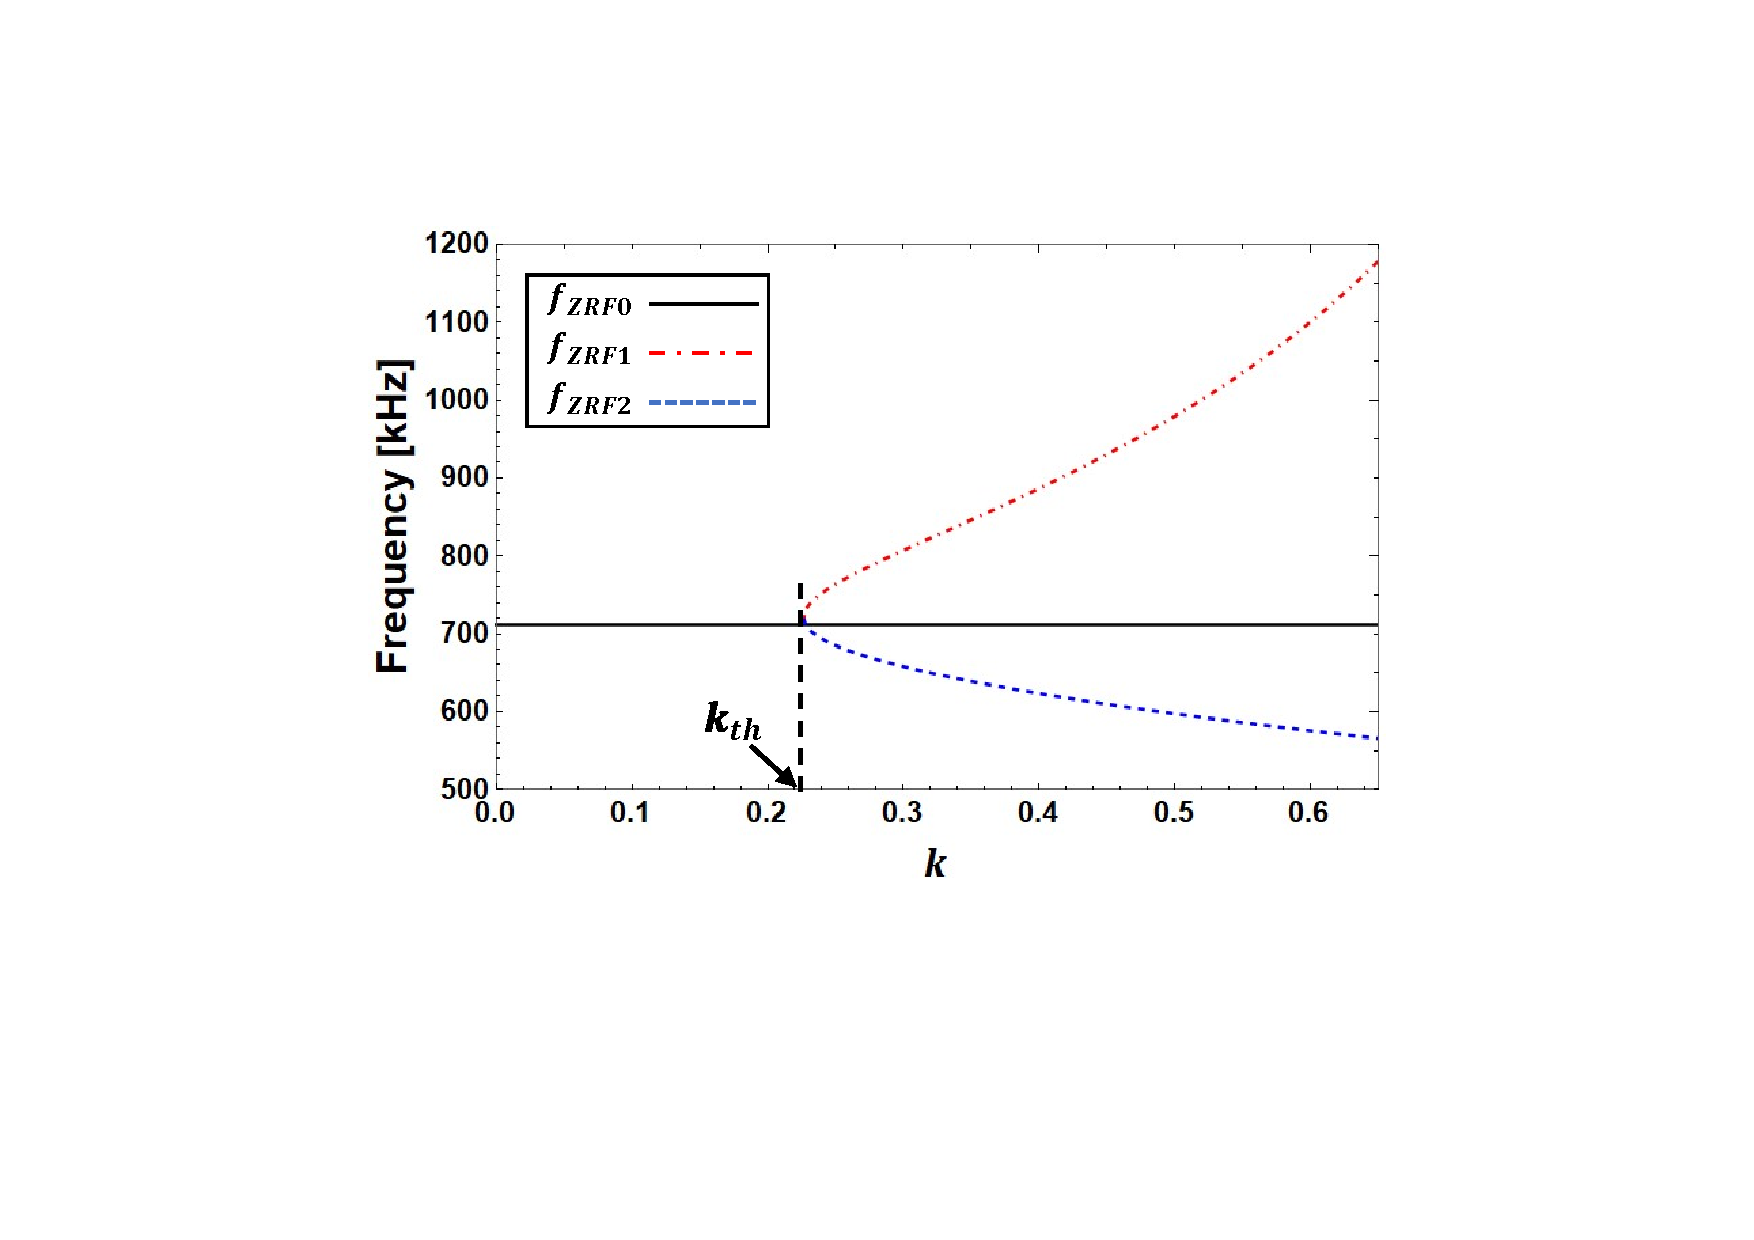
\includegraphics[width=100mm]{figures/zrfgraph.pdf}
		\caption{ZRFの理論曲線}
		\label{zrfgraph}
        \vspace{5mm}
        
		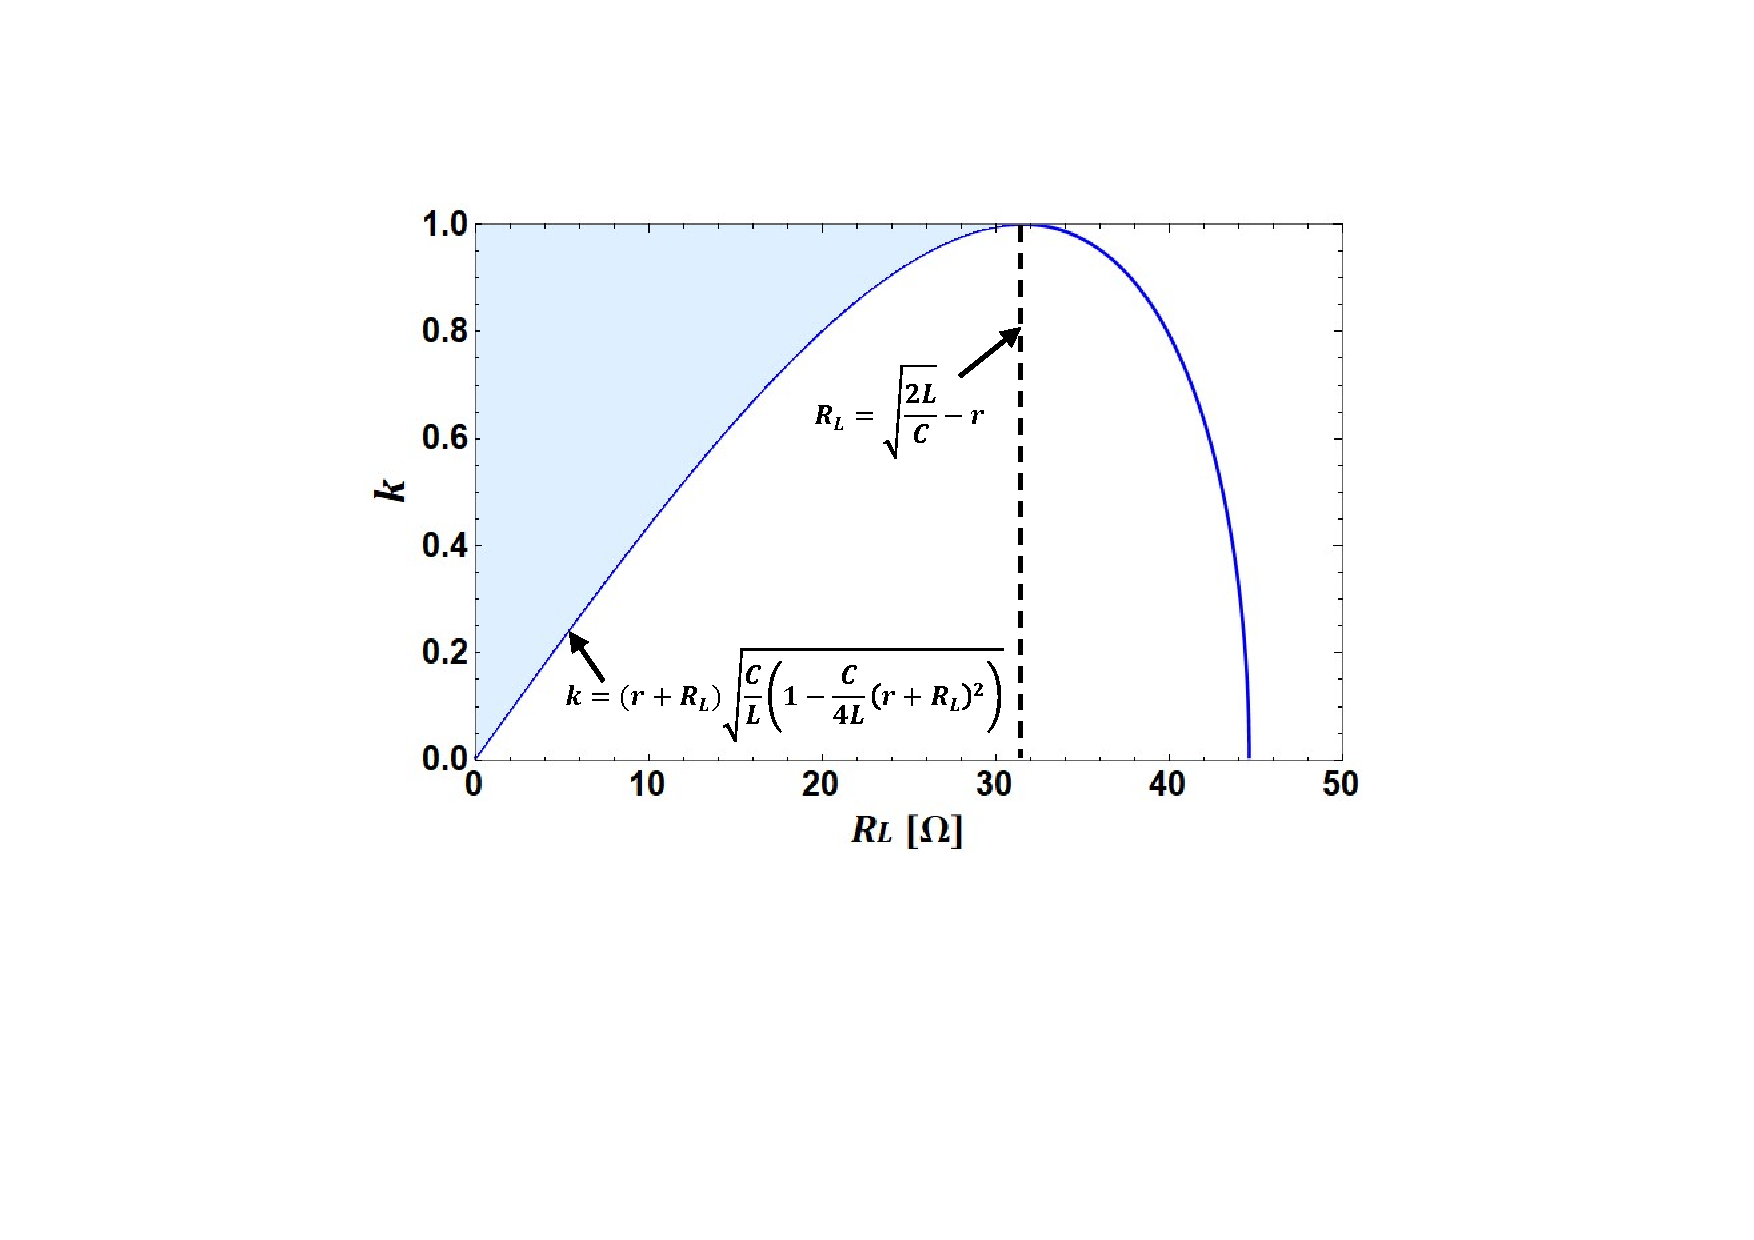
\includegraphics[width=100mm]{figures/boundary.pdf}
		\caption{ZRFが複数存在する条件}
		\label{boundary}

\end{center}
\end{figure}  
